\documentclass{article}
\usepackage{amsmath, amsthm, amsfonts, amssymb, geometry, graphicx, natbib}
\geometry{margin=2.5cm}

\title{LaTeX Eosystems Coursework Semester 2}
\author{Baciu Nichita}
\date{\today}


\begin{document}

\maketitle
\tableofcontents

\newpage

\section{Introduction}
Here is the introduction for the future exercises in LaTeX to show our skills. 

\subsection{Formatting Text}
This is the example of \textbf{bold} and \textit{italic} text.

\section{Mathematical Notation}
Example of the mathematical equation:

\begin{equation}
x_{1,2} = \frac{-b \pm \sqrt{b^2 - 4ac}}{2a}
\end{equation}


\section{BibTeX}
Here we can show how to make BibTeX reference using natbib: 

A rose by any other name would smell as sweet.\cite{Shakespeare}.
\bibliographystyle{plain}
\bibliography{references} 


\section{Table Example}
Here is an example of a table:

\begin{table}[h]
\begin{tabular}{|c|c|}
\hline
 Name & Age \\
\hline
Nichita & 19 \\
Bob & 21 \\
\hline
\end{tabular}
\end{table}

\section{Font families}
Here is the example of:\\
- Serif: \texttt{This is serif font.}\\
- Sans-serif: \textsf{This is sans-serif font.}\\
- Monospace: \texttt{This is monospace font.}\\

\section{Rulers}
Example of a full-width ruler:

\begin{center}
\hrulefill
\end{center}

\section{Spaces}
Examples of horizontal and vertical spaces:

Here is text \hspace{2cm} with a horizontal space.

Here is text \vspace{2cm}\\
With a vertical space

\section{Theorems and Proofs}
Pythagorean theorem.

\newtheorem{theorem}{Theorem}
\begin{theorem}
In a right triangle, the squared hypotenuse is equal to the sum of squared legs 
\end{theorem}

\begin{proof}
Given any right triangle with legs a and b and hypotenuse c like the above, use four of them to make a square with sides a+b as shown below:\\
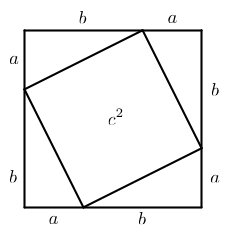
\includegraphics[width=0.2\textwidth]{pic-1.png}\\

This forms a square in the center with side length c and thus an area of \(c^2\) . However, if we rearrange the four triangles as follows, we can see two squares inside the larger square, one that is \(a^2\) in area and one that is \(b^2\) in area:\\
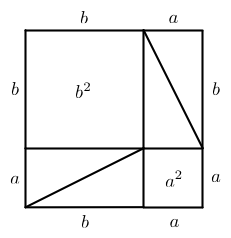
\includegraphics[width=0.2\textwidth]{pic-2.png}\\
Since the larger square has the same area in both cases, i.e. \((a+b)^2\) , and since the four triangles are also the same in both cases, we must conclude that the two squares \(a^2\) and \(b^2\) are in fact equal in area to the larger square \(c^2\) . Thus, \(a^2\) + \(b^2\) = \(c^2\).
\end{proof}

\end{document}
